\subsection{Efeitos Anisotrópicos do {\it Jet Quenching}} \label{ef_an}

Ao atravessar a matéria densa e quente, o parton perde energia e se resfria. A energia perdida
por este é depositada na matéria densa e quente, afetando a expansão hidrodinâmica do QGP
\cite{andrade_jet_2014}. Podemos observar estes efeitos na Figura \ref{fig:v2}.

\begin{figure}[!htb]
\centering
 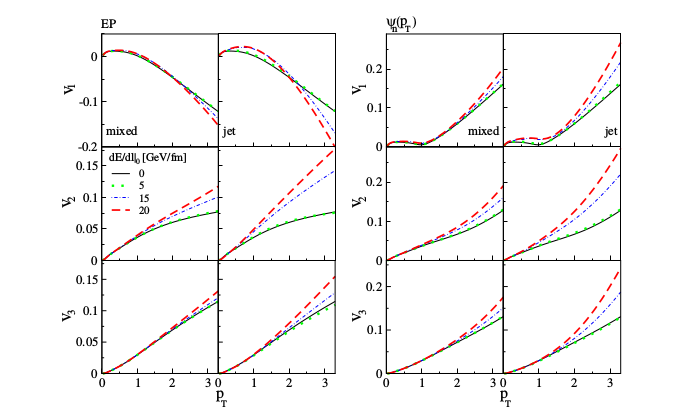
\includegraphics[scale=0.4]{Introducao/v2.png}
 \caption{Efeitos dos Jatos nos Harmônicos para diferentes valores de $p_{T}$.}
 \label{fig:v2}
\end{figure}

O estudo foi realizado basicamente com a inserão de um termo fonte nas equações hidrodinâmicas, da seguinte maneira:

\begin{equation}
 \partial_{\mu} T^{\mu \nu} = J^{\nu}
\end{equation}

O termo fonte foi construído conforme a equação:

\begin{equation}
 J^{\nu}(\tau,\overrightarrow{r}) = \sum_{n=1}^{n_p} \frac{s(\overrightarrow{r}^{jet}_{n}(\tau))}{s_0} \frac{dE}{dl}\bigg|_0
 F(\overrightarrow{r}-\overrightarrow{r}^{jet}_{n}(\tau),\tau;\sigma)(1,\overrightarrow{v}^{jet}_{n},0)
\end{equation}

A soma em questão é realizada sobre os partons viajando pela matéria densa. Os termos $s(\overrightarrow{r}^{jet}_{n}(\tau))$ e $s_0$
correspondem às entropias calculadas na posição do parton e em uma entropia de referência, respectivamente. A função $F$ corresponde a uma
distribuição Gaussiana representando o alcance do efeito do parton. E $\overrightarrow{v}^{jet}_{n}$ representa a velocidade do n-ésimo
parton.